\chapter{Ejemplos de aplicación}
\label{chap3}
\chapterquote
{The City's central computer told you? R2-D2, you know better than to trust a strange computer. }
{C-3PO, from Star Wars}

\section{Movimiento por fuerza boyante en un circuito cerrado}
\label{3:ff}

\subsection*{Presentación del problema}
Como primer ejemplo se presenta un sistema que se estudia analizándolo en dos subsistemas separados,
definiendo dos interfaces de acople,
y en cada una de ellas dos pares de variables dinámicas.
El primer subsistema modela un fluido en un tanque de paredes adiabáticas y con fuente interna de energía. 
El segundo subsistema representa un circuito en el que el fluido transfiere energía en un intercambiador de calor para bajar su temperatura.
Ambos se comunican mediante dos conexiones, una ubicada en la parte inferior y la otra en la parte superior,
definiendo un circuito cerrado en el que el flujo queda completamente dominado por convección natural.
El sistema completo modela el movimiento de un fluido en régimen de convección natural a través de
una fuente fría de neutrones alojada próxima al núcleo de un reactor de investigación \cite{fuente-fria}.
En la Figura \ref{esquemaFuenteFria} puede apreciarse un diagrama del sistema.

\begin{figure}[ht]
\centering{}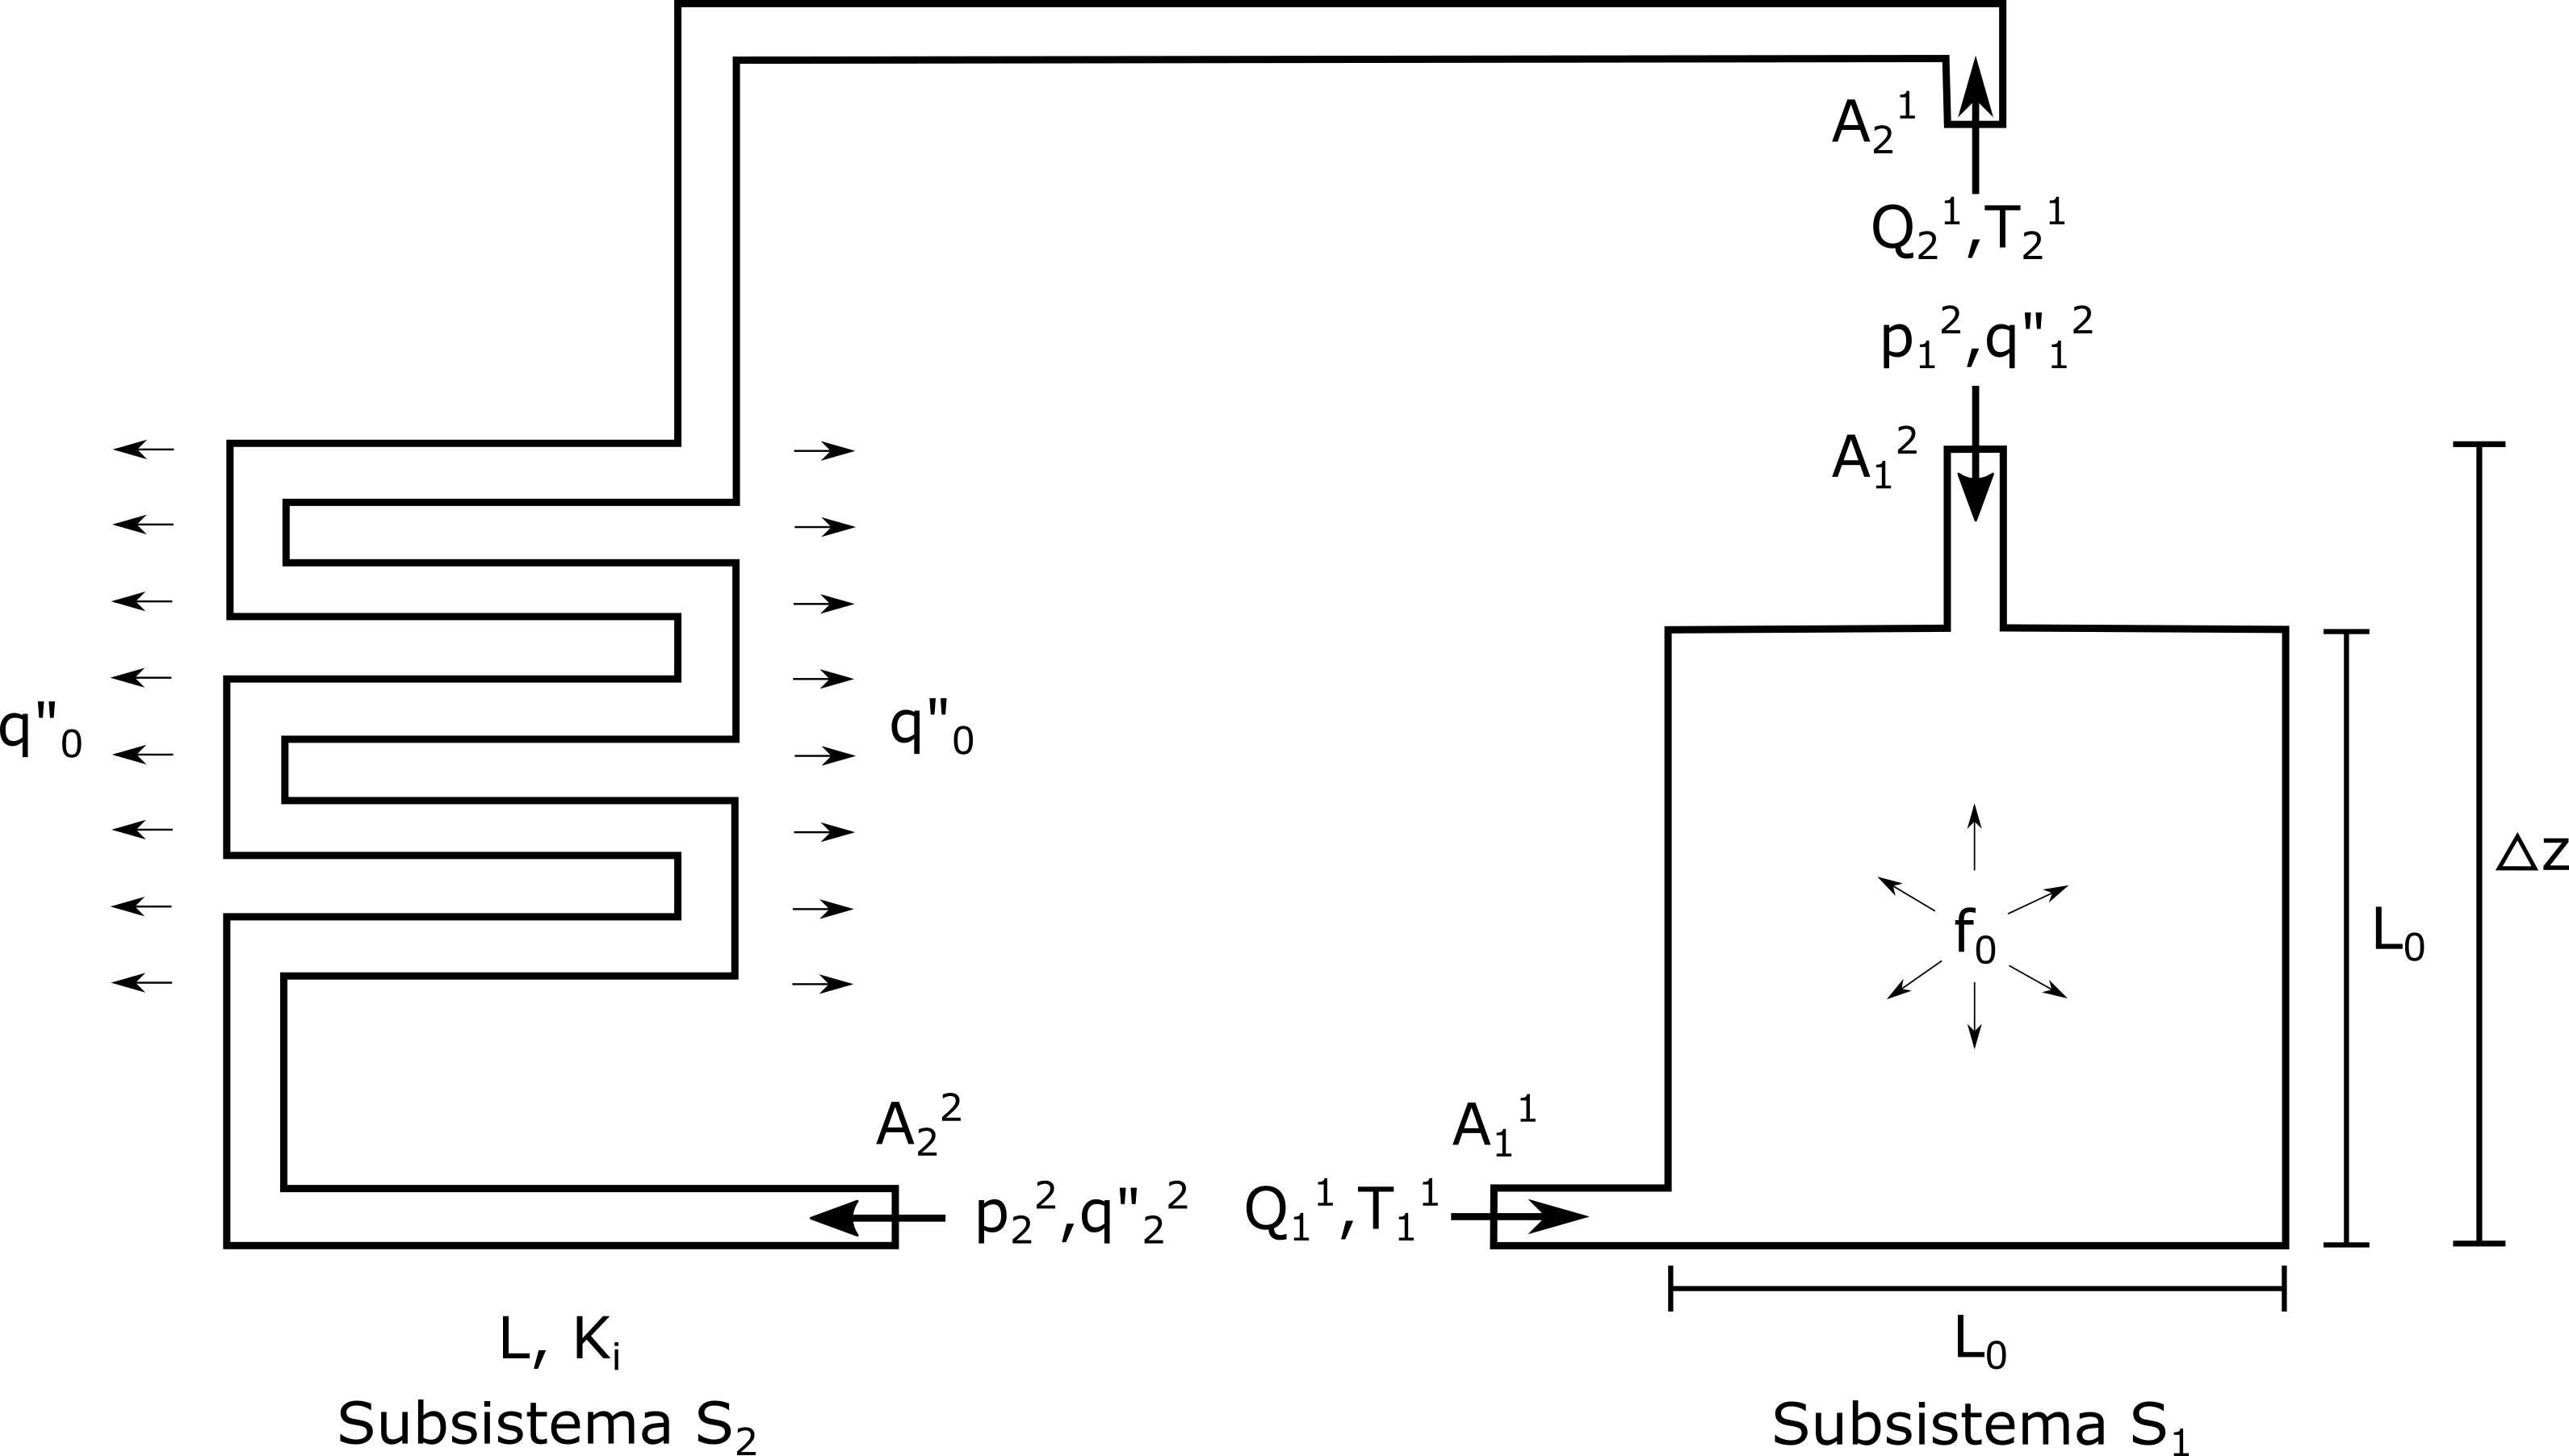
\includegraphics[scale = 0.25]{acople_ri_enief.png}
\caption{Esquema del sistema analizado. 
El subsistema de la izquierda es un intercambiador de calor y se estudia con un código cero-dimensional.
El modelo de la derecha es una cavidad con una fuente de energía interna y se estudia con un código bi-dimensional.
El sistema completo es abordado con una estrategia de acoplamiento mediante condiciones de borde dinámicas.
En el esquema se ejemplifica una de las elecciones posibles para las variables que son datos en cada subsistema.}
\label{esquemaFuenteFria}
\end{figure}

En cada interfaz de acople existen incógnitas de velocidades, fuerzas, temperatura y flujo de calor.
En el caso de las velocidades la estrategia implementada es definir una variable integral, 
el caudal volumétrico, que servirá como una de las variables de acoplamiento\footnote{
Cuando se utilizan variables integrales o promediadas para el acoplamiento, es necesario definir una estrategia extra en el subdominio que la recibe.
Como cada subproblema solo queda bien definido si la condición de borde está dada sobre todos los puntos del borde, estos valores deben distribuirse considerando algún perfil.
Por ejemplo, para el caso del subdominio que recibe un valor de caudal, y está modelado con ecuaciones bi-dimensionales, necesita definir un perfil de velocidades a lo largo de toda la sección de acople.
La definición del perfil se basa en alguna hipótesis que la persona que está modelando considera adecuada conforme a la física del problema.
Este paso debe analizarse con cuidado ya que los resultados del acoplamiento dependen de ello.
}.
En el caso de las fuerzas se utilizan valores promediados para la fuerza normal (presión).
Las fuerzas tangenciales se consideran nulas bajo la hipótesis de que son despreciables en las interfaces de acople.
Esta hipótesis es correcta cuando el flujo es paralelo, 
y por ello se selecciona como interfaz de acople aquella que se corresponda con el perfil de velocidades lo más plano posible, lejos de las curvas.
Los valores de temperatura de acople también corresponden a valores promediados en la interfaz,
y el flujo de calor corresponde al flujo integral a través de ella.
En los subsistemas bi-dimensionales, los perfiles de velocidadades y temperaturas construidos a partir de las variables recibidas se consideran planos,
bajo la hipótesis de flujo paralelo.
Con esta estrategia, existen cuatro incógnitas en cada interfaz de cada subsistema. 
Considerando los dos subsistemas, existen en total dieciseis incógnitas.
Por lo tanto el sistema queda definido por ocho ecuaciones de continuidad de campos de variables
y otras ocho ecuaciones de residuos que relacionan las incógnitas de forma similar 
a la que se presentó en la sección \ref{1:abordaje}.

Las ecuaciones de continuidad en las interfaces implican que:

\begin{equation}
\left\{ \begin{array}{rcl}
Q_1^1&=& Q_2^2 \\
Q_1^2&=& Q_2^1 \\
p_1^1&=& p_2^2 \\
p_1^2&=& p_2^1 \\
T_2^1&=& T_2^2 \\
T_2^2&=& T_2^1 \\
q"_2^1&=& - q"_2^2 \\
q"_2^2&=& - q"_2^1
\end{array}
\right.
\end{equation}
donde $Q$ es caudal, $P$ es presión, $T$ es temperatura y $q"$ es flujo de calor. 
Notar que el subíndice en cada variable refiere a la numeración global del subsistema, y el supraíndice indica el número de interfaz local,
como se convino previamente en el \hyperlink{chapter.1}{Capítulo 1}.
Al evaluar los residuos en cada interfaz, se genera una ecuación no lineal por cada incógnita en cada interfaz.
Para que las ecuaciones queden bien planteadas se selecciona solo una de las relaciones para el par presión-caudal
y solo una para el par temperatura-flujo de calor en cada interfaz.
Así entonces, entre las dos interfaces del subsistema 1 se generan cuatro ecuaciones de residuos
\footnote{
Cada ecuación de residuo relaciona las incógnitas según el modelo aplicado.
En $R_{p,Q}$ se considera dependencia entre el caudal $Q$, la presión $p$ y la temperatura $T$, y en 
$R_{T,q"}$ se considera dependencia entre el caudal $Q$, la temperatura $T$ y el flujo de calor $q"$.
} del tipo $(R_m)_{i}^{l}=0$:

%~ \begin{equation}
%~ \[
%~ \begin{Bmatrix*}
%~ (R_{p,Q})_{1}^{1}  \;(Q_1^1, p_1^1, T_1^1, q"_1^1, Q_1^2, p_1^2, T_1^2, q"_1^2) = 0 \\
%~ (R_{T,q"})_{1}^{1} \;(Q_1^1, p_1^1, T_1^1, q"_1^1, Q_1^2, p_1^2, T_1^2, q"_1^2) = 0 \\
%~ (R_{p,Q})_{1}^{2}  \;(Q_1^1, p_1^1, T_1^1, q"_1^1, Q_1^2, p_1^2, T_1^2, q"_1^2) = 0 \\
%~ (R_{T,q"})_{1}^{2} \;(Q_1^1, p_1^1, T_1^1, q"_1^1, Q_1^2, p_1^2, T_1^2, q"_1^2) = 0 
%~ \end{matrix*}\right
%~ \]
%~ 
%~ y entre las dos interfaces del subsistema 2 se generan otras 4 ecuaciones de residuos:
%~ 
%~ \[
%~ \begin{Bmatrix*}
%~ (R_{p,Q})_{2}^{1}  \;(Q_2^1, p_2^1, T_2^1, q"_2^1, Q_2^2, p_2^2, T_2^2, q"_2^2) = 0 \\
%~ (R_{T,q"})_{2}^{1} \;(Q_2^1, p_2^1, T_2^1, q"_2^1, Q_2^2, p_2^2, T_2^2, q"_2^2) = 0 \\
%~ (R_{p,Q})_{2}^{2}  \;(Q_2^1, p_2^1, T_2^1, q"_2^1, Q_2^2, p_2^2, T_2^2, q"_2^2) = 0 \\
%~ (R_{T,q"})_{2}^{2} \;(Q_2^1, p_2^1, T_2^1, q"_2^1, Q_2^2, p_2^2, T_2^2, q"_2^2) = 0
%~ \end{matrix*}\right
%~ \]
\begin{equation}
\left\{ \begin{array}{rcl}
(R_{p,Q})_{1}^{1}  \;(Q_1^1, p_1^1, T_1^1, Q_1^2, p_1^2, T_1^2) &=& 0 \\
(R_{T,q"})_{1}^{1} \;(Q_1^1, T_1^1, q"_1^1, Q_1^2, T_1^2, q"_1^2) &=& 0 \\
(R_{p,Q})_{1}^{2}  \;(Q_1^1, p_1^1, T_1^1, Q_1^2, p_1^2, T_1^2) &=& 0 \\
(R_{T,q"})_{1}^{2} \;(Q_1^1, T_1^1, q"_1^1, Q_1^2, T_1^2, q"_1^2) &=& 0 
\end{array}
\right.
\label{residuos-1}
\end{equation}
y entre las dos interfaces del subsistema 2 se generan otras cuatro ecuaciones de residuos:

\begin{equation}
\left\{ \begin{array}{rcl}
(R_{p,Q})_{2}^{1}  \;(Q_2^1, p_2^1, T_2^1, Q_2^2, p_2^2, T_2^2) &=& 0 \\
(R_{T,q"})_{2}^{1} \;(Q_2^1, T_2^1, q"_2^1, Q_2^2, T_2^2, q"_2^2) &=& 0 \\
(R_{p,Q})_{2}^{2}  \;(Q_2^1, p_2^1, T_2^1, Q_2^2, p_2^2, T_2^2) &=& 0 \\
(R_{T,q"})_{2}^{2} \;(Q_2^1, T_2^1, q"_2^1, Q_2^2, T_2^2, q"_2^2) &=& 0
\end{array}
\right.
\label{residuos-2}
\end{equation}

Notar que según la estrategia de acoplamiento seleccionada, algunas de las dependencias pueden anularse.
En la Figura \ref{esquemaFuenteFria} se presenta una estrategia en la que las condiciones de borde dinámicas son 
de tipo de tipo Dirichlet para la interfaz inferior de la cavidad y la interfaz superior del intercambiador de calor, 
y de tipo de tipo Neumann para las restantes.
Como el circuito es cerrado es necesario proveer un valor de referencia para la presión.
En la formulación desarrollada se fija un valor de presión aritrario en la interfaz superior del intercambiador de calor,
por lo que la ecuación $(R_{p,Q})_{2}^{1}=0$ queda descartada, y es sustituida por la siguiente:

\begin{equation*}
p_2^1 = 0.
\end{equation*}

\subsection*{Subsistemas de estudio}
Los parámetros del modelo del intercambiador de calor son los siguientes:
flujo de calor por unidad de superficie $q_0"=-2\cdot 10^5 W/m^2$, 
longitud de cañerías $L=30$ $m$, 
sumatoria de coeficientes de pérdida de carga concentrada $\sum K_i=1.72$, 
rugosidad de cañerías $\epsilon=0.5\cdot 10^{-3}$ $m$.
Las áreas de las interfaces de acople son $A_2^1=A_2^2=0.03$ $m^2$.
La altura total $\Delta z$ de este subsistema es equivalente a la de la cavidad bidimensional.
La evolución de las variables $\{p,Q,T,q"\}$ en el subsistema se calcula mediante un código cero-dimensional
que resuelve ecuaciones de pérdida de carga en una red hidráulica con flujo turbulento \cite{iedelchik}
y de transferencia de energía en un intercambiador de calor con flujo constante \cite{kays}:

\begin{equation}
\left\{ \begin{array}{rcl}
p_2^1 + \rho g \Delta z &=& p_2^2 + \rho \frac{1}{2} \left( \frac{Q_1^1}{A_2^1} \right)^2  \left( \frac {f_D L} {D} + \sum_i K_i \right) \\ [0.2cm]
\displaystyle T_2^2 &=& \displaystyle T_2^1 + 2 \frac {q_0" L}{\frac{D}{2} \frac{Q_1^1}{A_2^1}\rho c_p}
\label{eq-intercambiador}
\end{array}
\right.
\end{equation}
donde $f_D$ es el factor de Darcy de pérdida de carga distribuida y $D$ es el diámetro de la tubería.
En este modelo se supone que el flujo de calor es nulo en la dirección axial en cada interfaz de acople.
Esta aproximación es correcta ya que las interfaces se seleccionaron lejos de fuentes y sumideros, donde los gradientes de temperatura son despreciables.
Con este modelo, ninguna de las dos ecuaciones puede recibir valores de contorno \textit{Dirichlet} en ambas interfaces,
ya que los valores de caudal y temperatura en una interfaz determinan el valor en la otra.
Por lo tanto, en la estrategia de acoplamiento, la primera ecuación debe tener, o bien ambos contornos con condiciones de tipo \textit{Neumann}, 
o bien uno con condición de tipo \textit{Neuman} y otro con condición de tipo \textit{Dirichlet}.
La segunda ecuación debe tener uno de los bordes con condición de tipo \textit{Dirichlet} y otro con condición de tipo \textit{Neumann}.
Esta condición es necesaria a pesar de que el flujo de calor recibido no va a ser utilizado, basado en la hipótesis de que es despreciable.
Si el flujo de calor fuera efectivamente apreciable, debería cambiarse el modelo en la ecuación planteada.

La cavidad bidimensional se modela con $L_0=0.3$ $m$, y $A_1^1=A_1^2=0.03$ $m^2$.
El fluido de trabajo es agua ($\rho_0=10^3$ $Kg/m^3$, $\mu=6\cdot 10^{-4}$ $Kg/ms$, $c_p=4184$ $J/KgK$, 
$k=0.64$ $W/mK$, $\beta=0.44\cdot10^{-3}K^{-1}$)
con fuente interna $f_0=10^6$ $W/m^3$.
La evolución de las variables $\{p,Q,T,q"\}$ en este subsistema se calcula resolviendo las ecuaciones de Navier-Stokes {\cite{gunzburger}}
y de transporte de energía \cite{kays}. 
Se utiliza la aproximación de \textit{Boussinesq} considerando variaciones de densidad solo en el término de fuerza volumétrica:

\begin{equation}
\left\{ \begin{array}{rcl}
\displaystyle \frac {\partial \bar{u}}{\partial t} + ( \bar{u} \cdot \nabla) \bar{u}  + \frac {\nabla p}{\rho_0} - 
\nabla \cdot \left[ \left( \nu + \nu_T \right) \left( \nabla \bar{u} + \nabla \bar{u}^T \right) \right] && \\
- \left( 1- \beta (T-T_{ref}) \right)\bar{g} &=& 0 \\ [0.2cm]
\nabla \cdot \bar{u} &=& 0 \\ [0.2cm]
\displaystyle \frac {\partial T}{\partial t} + ( \bar{u} \cdot \nabla) T =0 - \frac {k}{\rho_0 c_p} \Delta T &=& \displaystyle \frac{f_0}{\rho_0 c_p}
\label{eq-cavidad}
\end{array}
\right.
\end{equation}
donde $\rho_0$ es la densidad del fluido a la temperatura de referencia $T_{ref}$.

Las ecuaciones (\ref{eq-cavidad}) se resuelven mediante una formulación de elementos finitos, 
con elementos lineales para aproximar los campos de presiones, velocidades y temperaturas, 
estabilizando con los métodos \textit{SUPG} \cite{supg} y \textit{PSPG} \cite{pspg}.
El método \textit{SUPG} (\textit{Streamline Upwind Petrov-Galerkin}) se utiliza para estabilizar problemas de transporte con alto número de \textit{Peclet} (\textit{Pe}).
El \textit{Pe} es un número adimensional que relaciona la velocidad de advección de un flujo y la velocidad de difusión, y está relacionado con el número de \textit{Reynolds} (\textit{Re}).
En las ecuaciones de \textit{Navier-Stokes}, el método estabiliza las evoluciones con alto \textit{Re},
y consiste en la adición de una difusividad extra en la dirección de las líneas de corriente.
El método \textit{PSPG} (Pressure Stabilizing Petrov-Galerkin) se utiliza para evadir la condición \textit{LBB},
que básicamente impone restricciones sobre los espacios de elementos utilizados en el problema de \textit{Stokes}.

Las paredes imponen condiciones de no deslizamiento para las ecuaciones de \textit{Navier-Stokes} y de flujo de energía nulo para la ecuación de energía.
En las interfaces de acople, deben definirse una serie de condiciones de borde.
En las ecuaciones de \textit{Navier-Stokes}, en cada interfaz pueden setearse valores de velocidades normales, suponiendo velocidades tangenciales nulas (bajo la hipótesis de flujo paralelo),
o valores de fuerzas normales (presión), suponiendo que las fuerzas tangenciales son nulas.
En la ecuación de energía, cada borde necesita o bien un perfil de temperaturas o bien un perfil de flujo de calor.
Los cálculos se realizaron implementando diferentes estrategias y verificando que los mismos convergieran.

La malla de cálculo se genera con \textbf{Gmsh} \cite{gmsh} y se discretiza el dominio en $43874$ elementos triangulares con un tamaño medio de arista de $\Delta x \approx 0.005m$. 

Como se mencionó previamente, no existe necesidad de que ambos códigos utilicen el mismo paso temporal de cálculo.
Sin embargo en ambos modelos se utiliza $\Delta t=0.01s$, debido a que ninguno requiere una mayor discretización temporal.

Los cálculos cero-dimensionales se realizan con un programa escrito para este propósito.
Los cálculos bi-dimensionales se realizan con \textbf{Par-GPFEP} (programa de elementos finitos de propósito general paralelizado, el nombre se debe a sus siglas
en inglés, \textit{Parallel General Purpose Finite Element Program})
desarrollado en el Departamento de Mecánica Computacional de la Comisión Nacional de Energía Atómica (\cite{gpfep}, \cite{pargpfep}).

\subsection*{Resultados del cálculo}

\begin{figure}[ht]
	\begin{minipage}{0.5\linewidth}
		\centering
		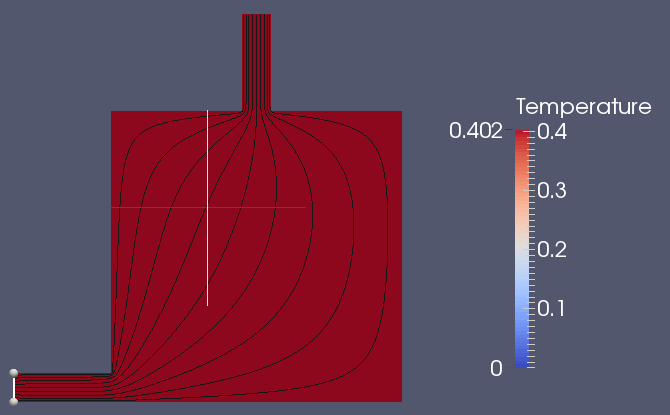
\includegraphics[scale=0.32]{acople_ri28_t0.png}
		\caption{t=0 s}
		\label{asd}	
	\end{minipage}
	\begin{minipage}{0.5\linewidth}
		\centering
		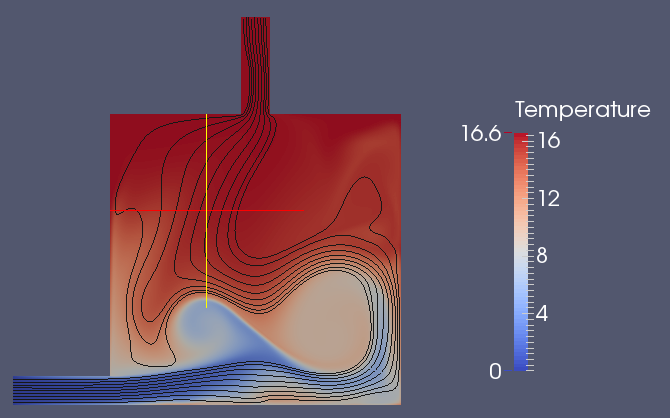
\includegraphics[scale=0.315]{acople_ri28_t40.png}
		\caption{t=40 s}
		\label{asd}	
	\end{minipage}
	\caption{Evolución del fluido dentro de la cavidad bidimensional con fuente interna.
	El número de Richardson del fluido $Ri=28.34$.
	Pueden apreciarse las líneas de corriente que se establecen al comienzo de la simulación.} 
	\label{acople_ri28_1}
\end{figure}

\begin{figure}[ht]
	\begin{minipage}{0.5\linewidth}
		\centering
		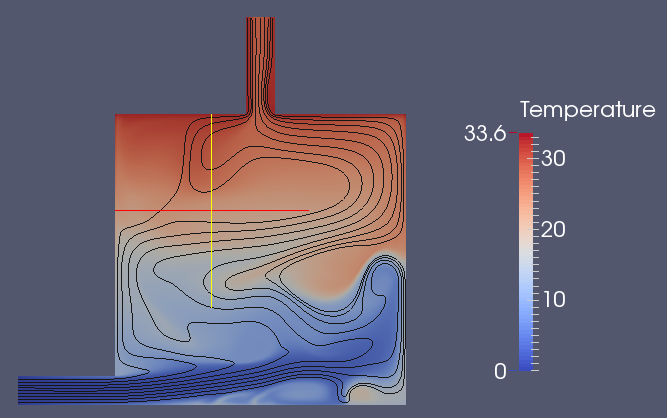
\includegraphics[scale=0.32]{acople_ri28_t80.png}
		\caption{t=80 s}
		\label{asd}	
	\end{minipage}
	\begin{minipage}{0.5\linewidth}
		\centering
		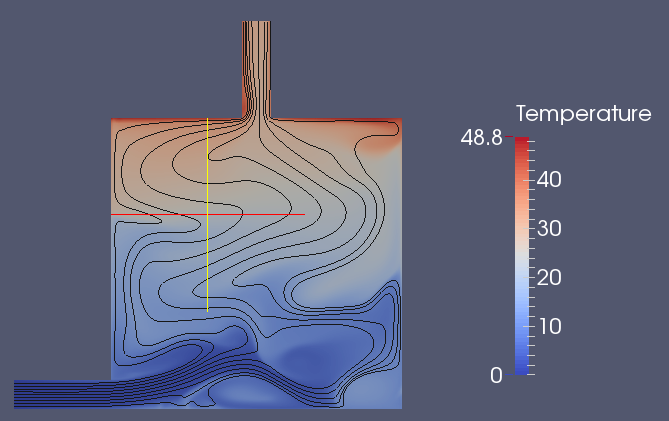
\includegraphics[scale=0.315]{acople_ri28_t250.png}
		\caption{t=250 s}
		\label{asd}	
	\end{minipage}
	\caption{Evolución del fluido dentro de la cavidad bidimensional con fuente interna.
	El número de Richardson del fluido $Ri=28.34$.
	Pueden apreciarse las líneas de corriente serpenteantes y la estratificación del fluido alcanzando un estado estacionario.}  
	\label{acople_ri28_2}
\end{figure}

Las condiciones iniciales del sistema son estáticas y sin gradientes de temperatura.
A medida que evoluciona el fluido comienza a incrementar su temperatura en la cavidad y a circular por fuerza boyante.
El régimen del fluido depende del número adimensional de Richardson \textit{Ri}, \cite{richardson},
que representa la relación entre las fuerzas boyantes y las fuerzas inerciales.
Con los parámetros del subsistema bidimensional el \textit{Ri} del fluido queda definido en $Ri=28.34$.
Como este valor es alto, el fluido se estratifica en capas de diferentes temperaturas.
Las líneas de corrientes serpentean entre la entrada y la salida, manteniendo corrientes paralelas horizontales.
En las Figuras \ref{acople_ri28_1} y \ref{acople_ri28_2} puede observarse 
la evolución de las líneas de corriente y del campo de temperatura en la cavidad bidimensional.

\subsection*{Análisis de métodos de resolución del sistema de ecuaciones de residuos}

Se exploran diferentes métodos numéricos para resolver el sistema de ecuaciones de residuos presentado en \ref{residuos-1} y \ref{residuos-2}.
En la Figura \ref{iteraciones_ri} puede apreciarse la cantidad de evaluaciones requeridas 
por cada método para disminuir los residuos debajo de cierta tolerancia prefijada, para cada paso temporal.
El método de \textit{Newton} calcula la matriz jacobiana en cada iteración.
Este cálculo se realiza con diferencias finitas a primer órden y por lo tanto requiere 1 evaluación de los residuos en el punto inicial, y 8 evaluaciones extras para el cálculo de cada diferencia finita.
En total son 9 evaluaciones extras.
Puede observarse que la cantidad de iteraciones del método para converger es en promedio una sola, ya que en general utiliza 10 evaluaciones en cada paso temporal.

\begin{figure}[ht]
\centering{}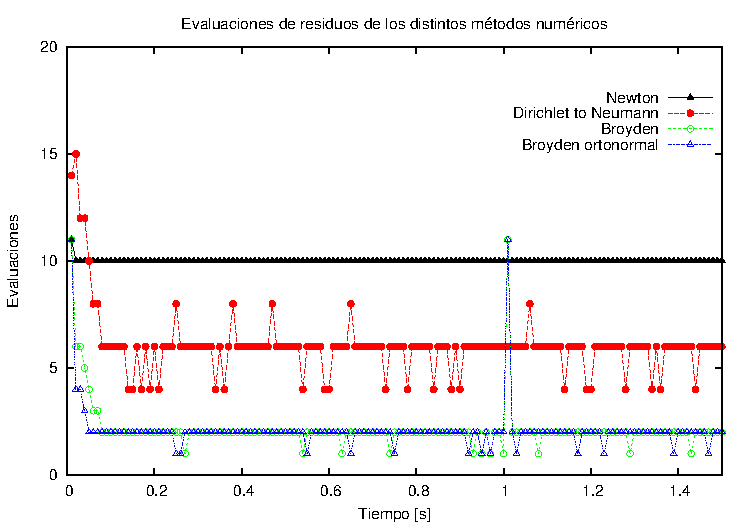
\includegraphics[scale = 1]{evaluaciones-ff.pdf}
\caption{Evaluaciones de residuos requeridas por diversos métodos numéricos para resolver los sistemas de ecuaciones planteados
 en el problema doblemente acoplado descripto de la fuente fría de neutrones.} \label{iteraciones_ri} 
\end{figure}

Los métodos \textit{quasi-Newton} inicializan la matriz jacobiana sólo en el primer paso temporal,
y luego utilizan aproximacionas económicas de la misma. 
Cada cierta cantidad de pasos temporales pueden reinicializar la matriz también mediante diferencias finitas. 
En los modelos realizados se utiliza reinicialización cada 100 pasos temporales, 
y por lo tanto la primera reinicialización se efectúa en el paso 101.
En promedio estos métodos requieren dos iteraciones por cada paso temporal, 
además de las 9 llamadas extras a códigos en cada paso de reinicialización.
Los métodos \textit{Broyden} y \textit{Broyden ortonormal} tinen comportamiento similar y demuestran ser más eficientes que el método clásico.
El método \textit{Dirichlet-to-Neumann} es el que mayor cantidad de iteraciones necesita por cada paso temporal, 
excediendo el doble de los pasos requeridos por los métodos \textit{quasi-Newton}.

\section{Análisis del segundo sistema de parada de un reactor de investigación}
\label{3:mock-up}

\subsection*{Presentación del problema}
El Departamento de Mecánica Computacional de CNEA tuvo a cargo el análisis del segundo sistema de parada (SSP) del reactor RA-10.
El SSP consiste en el accionamiento del vaciado del tanque reflector.
El drenado del material reflector (agua pesada) disminuye drásticamente la reactividad, apagando el reactor.
La tarea consistió en verificar si el diseño cumple con el criterio de éxito,
a saber, completar el 55\% del vaciado en un tiempo inferior a los 15 segundos,
ante una falla simple del sistema (falla de apertura de cualquiera de las válvulas).
Este requerimiento pudo verificarse tras el análisis \cite{cnea-informe-ra10}.

\begin{figure}[ht]
\centering{}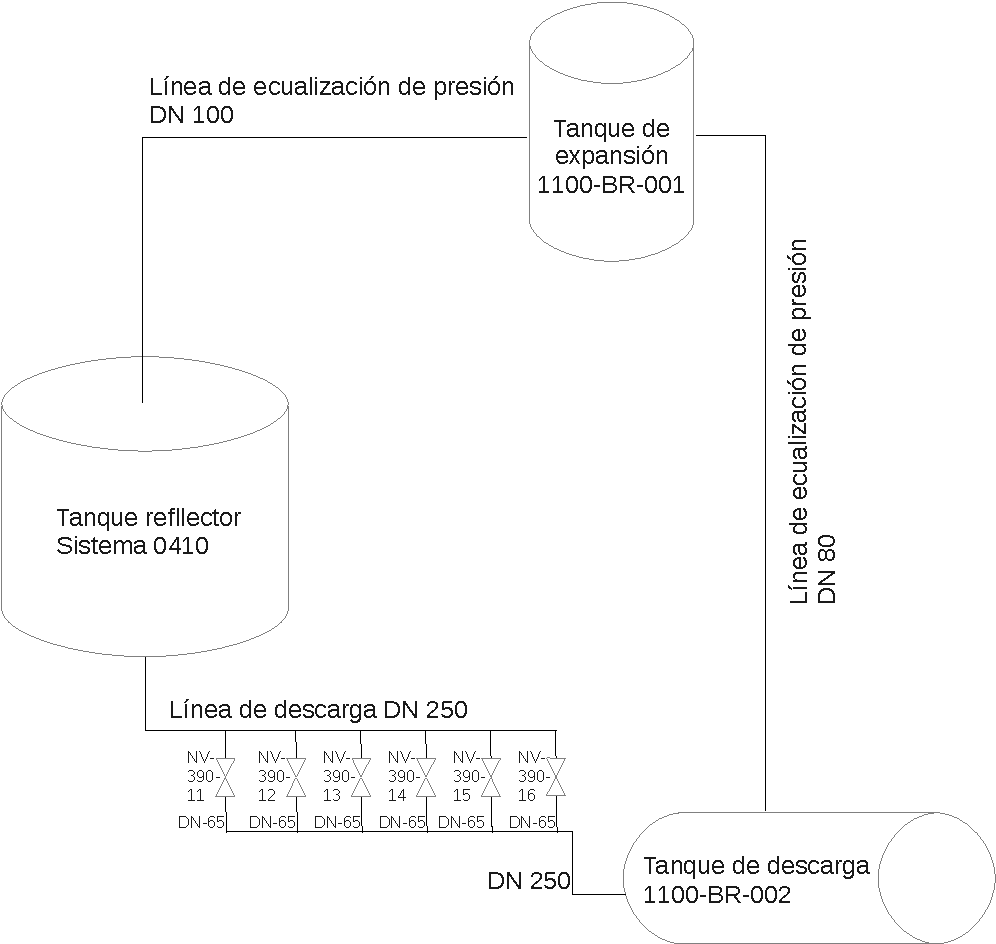
\includegraphics[scale = 0.8]{SSP.pdf}
\caption{Esquema del segundo sistema de parada del reactor RA10.} \label{fig:SSP} 
\end{figure}

La Figura \ref{fig:SSP} esquematiza el SSP. 
En el mismo pueden destacarse tres grandes subsistemas: el tanque del reflector, la red hidráulica de descarga y
la red hidráulica de ecualización de presiones. 
En operación normal del reactor las
válvulas que pueden observarse en la red hidráulica permanecen cerradas, y el agua pesada rellena las cañerías y el tanque de reflector. 
El resto del sistema es rellenado con gas Helio, excepto una porción del tanque de expansión que también permanece rellena con líquido. 
Cuando es accionado el SSP se abren las válvulas y el líquido comienza a drenar hacia el tanque de descarga, acelerado por la fuerza gravitatoria. 
Asimismo, el Helio circula en el mismo sentido en el resto del sistema, rellenando el volumen desplazado de líquido.

El análisis del problema completo hubiera demandado elevados recursos computacionales debido a los requerimientos de malla.
Por ello se propuso desarrollar un modelo multiescala del sistema,
desacoplándolo en subsistemas que pudieron estudiarse por separado con estrategias de acoplamiento mediante condiciones de borde apropiadas.
El SSP del RA10 se dividió en tres subsistemas:

\begin{itemize}
\item Subsistema del tanque del reflector,
\item Subsistema de la red hidráulica de descarga,
\item Subsistema de la red hidráulica de ecualización de presiones.
\end{itemize}

En el trabajo presentado los subsistemas se acoplaron mediante una estrategia de acoplamiento débil \cite{ra10-paper} \cite{ra10-enief}.
Durante el trabajo se realizaron tareas de validación de las herramientas de cálculo.
Para ello se estudió un sistema similar para el que se conocían datos experimentales de tiempo de vaciado.
Estos datos sirvieron para contrastar los resultados obtenidos con las herramientas de cálculo.
El sistema analizado fue el tanque del reflector del mockup del reactor OPAL, 
montado por INVAP en San Carlos de Bariloche, \cite{invap-mockup}.

Debido a que el mockup del OPAL está abierto a la atmósfera, no cuenta con línea de ecualización de presiones y por lo tanto no se consideró en el modelo.

En un estudio \cite{cnea-informe-mockup} se analizó el detalle fluídico tridimensional en el tanque reflector durante la descarga,
modelando con ecuaciones cero-dimensionales la pérdida de carga en la red hidráulica 
y acoplando los subsistemas de forma débil.
En el estudio aquí presentado se analiza con mayor detalle la distribución de caudales a través del arreglo de válvulas,
modelando el comportamiento del resto del sistema con ecuaciones cero-dimensionales.
El propósito de este estudio es investigar si existe algún efecto que podría no estar siendo considerado en el otro modelo.

\subsection*{Subsistemas de estudio}

Se proponen dos subsistemas de estudio:
el primero incluye el tanque del reflector acoplado a una porción de la red hidráulica en la descarga,
y el segundo modela el arreglo de válvulas.
Ambos están conectados a través de una sección de la tubería,
en la cual quedan acoplados los valores de velocidades y fuerzas.
La estretegia implementada es similar a la utilizada en \ref{3:ff} ya que se utilizan como variables de acoplamiento el caudal volumétrico y la presión promedio.
Las fuerzas tagenciales se consideran nulas.
A fines de cumplir con esta hipóteisis, la interfaz de acople se selecciona lejos de los codos.
El subsistema tanque del reflector tiene como incógnitas la presión $p_1^1$ y el caudal $Q_1^1$ en la interfaz de acople $I_1^1$.
Asimismo, el subsistema arreglo de válvulas tiene como incógnitas $p_2^1$ y $Q_2^1$ en $I_{2_1}$.
Las ecuaciones de continuidad implican que:

\begin{equation}
\left\{ \begin{array}{rcl}
p_1^1 &=& p_2^1 \\
Q_1^1 &=& Q_2^1
\end{array}
\right.
\end{equation}

Se utiliza la siguiente estrategia:
condiciones de borde de tipo \textit{Neumann} en la interfaz de acople para el subsistema tanque del reflector,
y condiciones de borde de tipo \textit{Dirichlet} para el subsistema arreglo de válvulas\footnote{
Se podrían haber definido otras estrategias.
La estrategia implementada permite resolver las ecuaciones en ambos subdominios de una forma cómoda.
En el modelo tri-dimensional, por ejemplo, el valor de caudal recibido es útil para construir valores para las condiciones de borde del modelo turbulento utilizado.
}.
En base al caudal recibido en este subsistema se calcula un perfil de velocidades.
Las ecuaciones de residuos quedan entonces:

\begin{equation}
\left\{ \begin{array}{rcl}
(R_{p,Q})_{1}^{1}  \;(p_1^1) &=& 0 \\
(R_{p,Q})_{2}^{1}  \;(Q_2^1) &=& 0
\end{array}
\right.
\end{equation}

El primer subsistema se analiza con ecuaciones cero-dimensionales,
realizando balances de masa y energía.
La evolución de la altura $h$ de la superficie libre en el tanque del reflector
queda modelada a través de la siguiente ecuación \cite{bird}:

\begin{equation}
\ddot{h} h + \frac{\dot{h}^2}{2}\left( 1- \left(\frac{A_T}{A_D} \right)^2 \right) + g \Delta h_{red} + \ddot{h}  l_D = 
\frac{p_{atm}-p_1^1}{\rho} + \Delta \hat{u}
\label{eq-tanque}
\end{equation}
donde $p_1^1$ es la presión en la interfaz de acople,
que se recibe como dato de contorno,
$A_T$ es la área transversal del tanque del reflector, 
$A_D$ es la sección transversal de la línea de descarga,
$\Delta h_{red}$ es la altura total de la columna de líquido en el subsistema,
$l_D$ es la longitud total de cañerías en el subsistema,
$p_{atm}$ es la presión sobre la superficie libre,
y $\rho$ es la densidad del agua.
$\Delta u$ representa la pérdida de carga por unidad de masa y puede modelarse como:

\begin{equation}
\Delta u = \frac {1} {2} {v_D}^2 \left( \frac {f_D l_D}{D} + \sum_i K_i \right)
\end{equation}
donde $v_D$ es la velocidad del fluido en la línea de descarga,
(que puede escribirse en términos de $\dot{h}$),
$\frac {f_D*l_D}{D}$ es el factor de pérdida de carga distribuida en las tuberías,
(en función del factor de Darcy $f_D$, la longitud de tuberías $l_D$ y el diámetro de las mismas $D$)
y $\sum_i K_i$ es la sumatoria de factores de pérdida de carga concetrada.

CB

La Tabla \ref{tabla-tanque} reúne los parámetros del subsistema.
Los datos geométricos pueden consultarse en las referencias \cite{invap-mockup}.
El factor de pérdida de carga concentrada fue calculado en función de estos datos geométricos \cite{iedelchik},
e incluye la contracción abrupta en la unión entre el tanque y la red hidráulica,
y tres codos de 90º presentes en ella, previos al arreglo de válvulas.

\begin{table}[]
\centering
\begin{tabular}{|l|l|}
\hline
Parámetro        & Valor          \\ \hline
$A_T$            & 5.30 $m^2$     \\ \hline
$A_D$            & 0.05 $m^2$     \\ \hline
$\Delta h_{red}$ & $h$ + 4.98 $m$ \\ \hline
$l_D$            & 11.98 $m$      \\ \hline
$p_{atm}$        & 92000 $Pa$     \\ \hline
$\rho$           & 998 $Kg/m^3$   \\ \hline
$D$              & 0.254 $m$      \\ \hline
$\sum_i K_i$     & 1.13           \\ \hline
\end{tabular}
\caption{Parámetros del subsistema del tanque del reflector con acople de sección de red hidráulica}
\label{tabla-tanque}
\end{table}

Una vez resuelta la ecuación (\ref{eq-tanque}) para un dado valor de tiempo,
el caudal de descarga $Q_1^1$ puede calcularse simplemente como:

\begin{equation}
Q_1^1 = -\dot{h} A_D
\label{eq-qd}
\end{equation}

El subsistema arreglo de válvulas es modelado con una malla tridimensional de elementos tetraédricos realizada en \textbf{Salomé} \cite{salome}.
El caudal ingresa a través del extremo superior y se reparte entre los múltiples caños que comunican los colectores.
En operación normal del reactor cada uno de ellos está bloqueado mediante una válvula esférica,
y del otro lado las cañerías están rellenas de gas,
pero durante el accionamiento del sistema de parada las mismas se abren dejando pasar libremente al fluido.
Las válvulas esféricas instaladas no presentan pérdidas de carga concentrada y por lo tanto no son modeladas.
Como es de interés el análisis ante falla simple del sistema,
se supone que una de las válvulas no abre y por ello ese caño tampoco se modela.
En los primeros cálculos se supone que la válvula en falla es la ubicada en la última rama del arreglo.
Como otra simplificación del problema se supone que inicialmente el agua rellena todas las cañerías en forma estática.
Más adelante se estudia la validez de éstas aproximaciones.
Los datos dimensionales de las cañerías pueden consultarse en las referencias \cite{invap-mockup}.

Debido a que el régimen del fluido es turbulento durante la mayor parte de la descarga,
y una simulación DNS demandaría elevados recursos computacionales,
se utiliza un modelo de turbulencia de tipo RANS para modelar la fricción interna del fluido.
El modelo utilizado es el modelo $\kappa-\epsilon$ \textit{realizable}, en el que
las ecuaciones se estabilizan mediante un método de control de coeficientes \cite{k-e-realizable}.
El sistema de ecuaciones resultantes en el segundo subsistema es:

\begin{equation}
\left\{ \begin{array}{rcl}
\displaystyle \frac{\partial \bar{U} }{\partial t} + ( \bar{U} \cdot \nabla) \bar{U} + \frac {\nabla P^*}{\rho} - 
\nabla \cdot \left[ \left( \nu + \nu_T \right) \left( \nabla \bar{U} + \nabla U^T \right) \right] -\bar{f} &=& 0 \\
\nabla \cdot \bar{U} &=& 0 \\
\displaystyle \nu_T -c_\mu \frac{\kappa^2}{\epsilon} &=& 0\\
\displaystyle \frac{\partial \kappa}{\partial t} + ( \bar{U} \cdot \nabla) \kappa - \frac{c_\mu} {2}{\kappa^2}{\epsilon} \left | \nabla \bar{U} + \nabla\bar{U}^T \right | ^2  
- \nabla \cdot \left( c_\mu \frac{\kappa^2}{\epsilon} \nabla \kappa \right) + \epsilon &=& 0 \\
\displaystyle \frac{\partial {\epsilon}}{\partial t} + ( \bar{U} \cdot \nabla) \epsilon - \frac{c_1} {2} \kappa \left | \nabla \bar{U} + \nabla \bar{U}^T \right | ^2
- \nabla \cdot \left( c_{\epsilon} \frac{\kappa^2}{\epsilon} \nabla \epsilon \right) + c_2 \frac{\epsilon}{\kappa} &=& 0
\label{eq-mani}
\end{array} \right.
\end{equation}
donde $\bar{f}$ es una fuerza volumétrica, 
$\kappa$ es la energía cinética turbulenta, $\epsilon$ es la disipación viscosa de energía turbulenta,
$\nu_T$ es la viscosidad turbulenta y $P^*$ es la presión efectiva del sistema, que se calcula como
$\displaystyle P^* = P + \frac {2}{3}\kappa$.
Las variables mayúsculas refieren a valores medios estadísticos.
Los parámetros de las ecuaciones de transporte de $\kappa$ y $\epsilon$ toman los siguientes valores:
$c_\mu=0.09$, $c_1=0.126$, $c_2=1.92$ y $c_\epsilon=0.07$ \cite{durbin}.

En las ecuaciones de \textit{Navier-Stokes}, cada borde necesita un perfil de velocidades normales o de fuerzas normales,
y otro de velocidades tangenciales o de fuerzas tangenciales \cite{gunzburger}.
Las condiciones de borde al ingreso de la cañería dependen del valor $Q_2^1$ impuesto,
a partir del cual se define un perfil de velocidades plano del fluido.
En base a estas velocidades se calcula un valor para la intensidad turbulenta $I_T$,
y con ella se aproximan los valores de $\kappa$ y $\epsilon$ en la interfaz.
En la descarga de la cañería se impone una fuerza normal que depende de la presión atmosférica,
despreciando las fuerzas tangenciales.
Las ecuaciones de $\kappa$ y $\epsilon$ no requieren condiciones contorno en esta interfaz.
Para evitar la resolución de la capa límite en las paredes de las tuberías se implementa un modelo de pared,
en el que se reemplaza la misma por una tracción tangencial equivalente a la que realizaría la misma sobre la corriente externa
\cite{k-e}.
Este modelo impone condiciones de tipo \textit{Dirichlet} para $\kappa$ y $\epsilon$ en la frontera en que se impone la ley de pared.

El sistema de ecuaciones (\ref{eq-mani}) es resuelto en pasos fraccionados \cite{lew} mediante una formulación de elementos finitos con elementos lineales, 
estabilizada mediante \textit{SUPG} \cite{supg} y \textit{PSPG} \cite{pspg}.
En el primer paso fraccionado se resuelve el transporte de $\kappa$,
en el segundo paso se resuelve el transporte de $\epsilon$,
y en el último paso se resuelven en forma monolítica las ecuaciones de \textit{Navier-Stokes}.

Una vez resueltas las ecuaciones es posible calcular el valor de la presión promedio $<p_2^1>$ en la interfaz $I_{2_1}$,
a partir de los valores $<P^*_{I_2^1}>$ y $<\kappa_{I_2^1}>$ promediados en ella:

\begin{equation}
<p_2^1> = <P^*_{I_2^1}> - \frac {2}{3} <\kappa_{I_2^1}>
\end{equation}

Los cálculos cero-dimensionales se realizan con un programa escrito para este propósito.
Los cálculos tri-dimensionales se realizan con \textbf{Par-GPFEP}.

\subsection*{Resultados del cálculo}

Se realizan cálculos utilizando mallas del modelo tri-dimensional con diferente refinamiento para estudiar la convergencia de los resultados.
La primera es una malla con $\Delta x=0.01m$ y 1145659 de elementos. 
La segunda es malla tiene $\Delta x=0.008m$ y 1806202 elementos.
La tercera es la malla más fina y tiene $\Delta x=0.005m$ y 2951259 elementos.
Se utiliza $\Delta t=0.01s$ en los cálculos con las dos primeras mallas y $\Delta t=0.005s$ en los cálculos con la última malla.
Las ecuaciones de residuos se resuelven estudiando diferentes métodos numericos.
mediante el método de Broyden ortonormal, 
con reinicialización de la matriz jacobiana cada 100 pasos temporales.
En la Figura \ref{qpvst} se reportan los resultados obtenidos para la evolución de los caudales y de las presiones en la interfaz de acople.

\begin{figure}[ht]
	\begin{minipage}{0.5\linewidth}
		\centering
		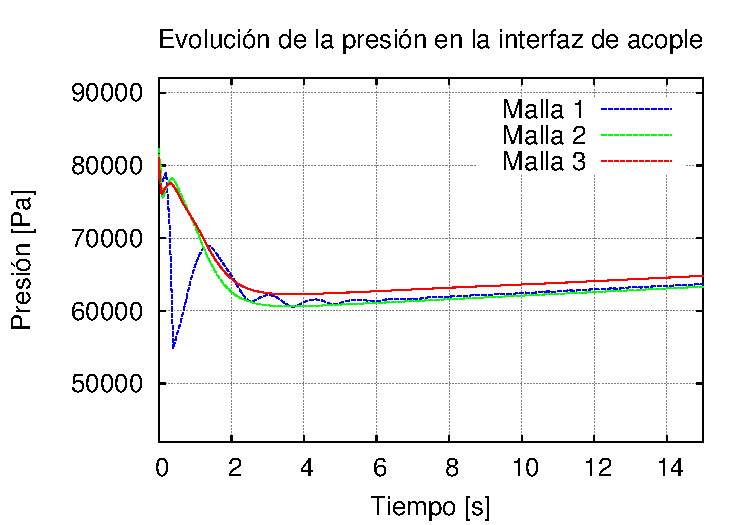
\includegraphics[scale=0.55]{p_vs_t.pdf}
		%\caption{t=80 s}
		\label{asd}	
	\end{minipage}
	\begin{minipage}{0.5\linewidth}
		\centering
		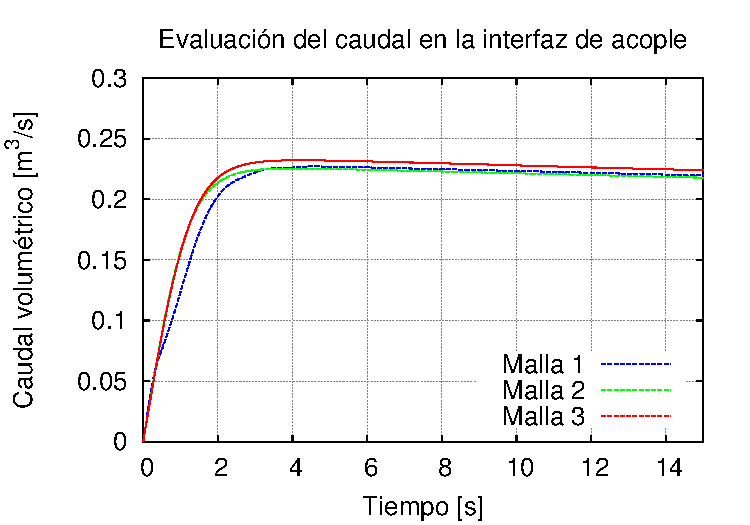
\includegraphics[scale=0.55]{q_vs_t.pdf}
		%\caption{t=250 s}
		\label{asd}	
	\end{minipage}
	\caption{Evolución de la presión y del caudal volumétrico en la interfaz de acople entre los dos subsistemas.
  La presión atmosférica es de 92000 Pa.}  
	\label{qpvst}
\end{figure}

%~ \begin{figure}[ht]
%~ \centering{}\includegraphics[scale = 1]{qpvst.pdf}
%~ \caption{Evolución de la presión y del caudal volumétrico en la interfaz de acople entre los dos subsistemas.}
%~ \label{qpvst}
%~ \end{figure}

En la Figura \ref{hvst} se observa la evolución de la altura de la superficie libre del líquido en el tanque durante los primeros quince segundos obtenida en diferentes cálculos.
La curva azul reporta los resultados obtenidos con la malla más gruesa, la curva roja los resultados obtenidos con la malla intermedia y la curva violeta los resultados obtenidos con la malla más fina.
La curva verde muestra resultados de análisis estudiando la condición inicial de gas de relleno en las cañerías, que será comentada en la sección \ref{3:level-set}.
Las curvas cyan y gris muestran resultados del cálculo del modelo tri-dimensional del tanque con acoplamiento débil al modelo cero dimensional de la red hidráulica \cite{ra10-paper},
obtenidas sin utilizar modelo de turbulencia, y utilizando el modelo \textit{RANS} previamente comentado.
Comparativamente se muestran también los valores experimentales reportados en la referencia \cite{invap-mockup}.

\begin{figure}[ht]
\centering
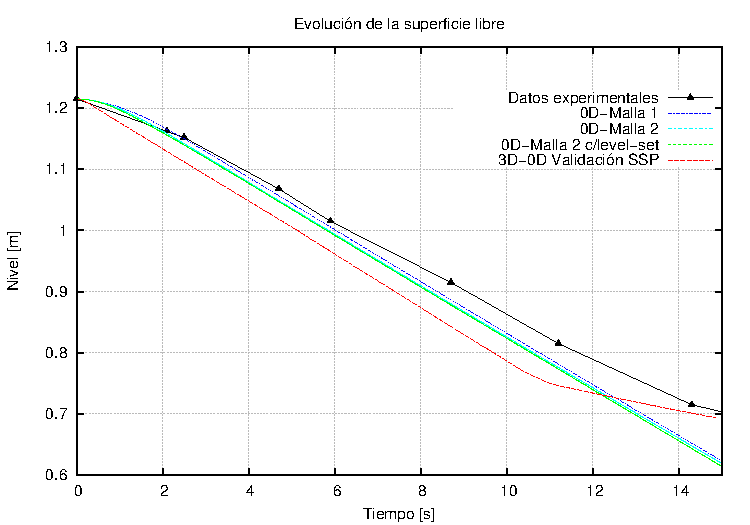
\includegraphics[scale = 1]{hvst.pdf}
\caption{Evolución del nivel de líquido en el mockup del tanque del reflector ante accionamiento del SSP.
La curva negra está construida con datos experimentales proporcionados por INVAP S.E.
Las curvas azul, roja, verde y violeta reportan datos calculados mediante diferentes mallas para el modelo tri-dimensional del arreglo de válvulas, 
con acoplamiento fuerte al modelo cero-dimensional del resto del sistema.
Las curvas cyan y gris muestran resultados del cálculo del modelo tri-dimensional del tanque con acoplamiento débil al modelo cero dimensional de la red hidráulica.}
\label{hvst} 
\end{figure}

Los modelos computacionales predicen un comportamiento dinámico similar al reportado experimentalmente.
Durante los primeros segundos de evolución existe una cierta inercia en la descarga que solo es captada por los modelos que describen el detalle en el arreglo de válvulas.
Tras este transitorio inicial, todos los modelos predicen una pendiente de vaciado similar.
Esta pendiente se corresponde con similares caudales de descarga entre los diferentes modelos, 
con lo que se verifica que la pérdida de carga total considerada en dos modelos independientes (modelo tri-dimensional del tanque acoplado, y modelo cero-dimensional del tanque acoplado) es similar.
La curva experimental presenta ciertas ondulaciones que se deben al efecto que el oleaje en la superficie del líquido genera sobre el punto de medición.
Estas variaciones son filtradas en el modelo tri-dimensional del tanque ya que la curva reporta una altura efectiva, calculada a partir del volumen restante de líquido en el tanque.
Transcurridos los diez segundos de descarga, existe un quiebre en las curvas del modelo tri-dimensional del tanque.
Este quiebre se corresponde al momento en el que las cañerías succionan tanto gas que es posible desacoplar el modelo cero-dimensional de pérdida de carga,
basándose en la hipótesis de que se establece una vena gaseosa entre el punto de succión y el orificio de descarga.
Esta hipótesis es conservativa para el objetivo de estudio previsto,
ya que si el acoplamiento de la red no fuera realmente despreciable, el tanque se vaciaría a mayor velocidad que la modelada.
En el tanque existe un cajón que envuelve la entrada a la red hidráulica y no permite el vaciado más allá de los 60 cm,
por lo que el nivel de líquido, que es medido fuera de este cajón, tiende asintóticamente a este valor.
Esta dinámica no es considerada en el modelo cero-dimensional del tanque, lo que explica las diferencias entre las curvas en los últimos segundos.

\subsection*{Análisis de sensibilidad de resultados ante válvula en falla}

Los cálculos previos se realizaron suponiendo que falla la válvula de la última conexión entre los colectores.
Es de interés conocer si existe variación en los tiempos de descarga si la válvula que falla es alguna otra.
En la Figura \ref{hvstv} se compara la evolución de la superficie libre ante fallas en la primera, la tercera y la sexta válvula.

\begin{figure}[ht]
\centering
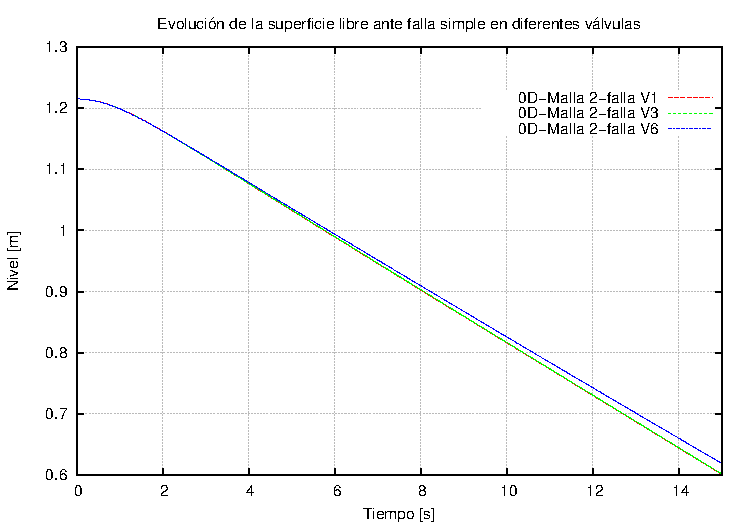
\includegraphics[scale = 1]{hvstv.pdf}
\caption{Comparación de la evolución del nivel de líquido en el mockup del tanque del reflector
ante accionamiento del SSP considerando falla simple en diferentes válvulas.}
\label{hvstv} 
\end{figure}

Como puede observarse no es posible notar diferencias considerables en la evolución de la descarga.
La pérdida de carga total del arreglo de válvulas es levemente sensible a la válvula que falla.

\subsection*{Transporte de superficie libre en las tuberías}
\label{3:level-set}

Como se comentó, en los cálculos realizados previamente no se consideró el gas de relleno en las tuberías durante los primeros instantes del drenado.
Es de interés estudiar su influencia.
Se utiliza la técnica de level-set para transportar la superficie libre \cite{level-set}.
Para ello se añade un paso fraccionado extra al sistema de ecuaciones (\ref{eq-mani}):

\begin{equation}
\left\{ \begin{array}{rcl}
\displaystyle \frac{\partial\phi}{\partial t}+ (\bar{u} \cdot \nabla) \phi &=& 0
\label{eq-ls}
\end{array} \right.
\end{equation}
donde $\phi$ es el campo que representa la distancia con signo de cada punto a la superficie libre.
Las porciones del sistema con líquido tienen $\phi$ positivo y las porciones con gas tienen $\phi$ negativo.
$\phi$ tiene valor nulo en la superficie libre.
La ecuación (\ref{eq-ls}) requiere un valor de contorno allí donde $\bar{u} \cdot \bar{n} < 0$,
y por lo tanto debe proveerse el valor del campo a la entrada de la tubería.
Esta ecuación también es resuelta mediante una formulación de elementos finitos con elementos lineales y estabilización \textit{SUPG}.
Se utiliza, además, un enriquecimiento del espacio de presiones en los elementos de la interfaz \cite{enriq}.
El campo del level set es reinicializado mediante cálculos geométricos cada 10 pasos temporales.

En la Figura \ref{hvst} se compara la evolución obtenida de la superficie libre con los resultados anteriores,
y en la Figura \ref{hvstls} se compara la evolución durante el transitorio inicial.
Puede observarse que al modelar el transporte del gas la descarga se acelera durante el primer instante, debido a la menor pérdida de carga.
Sin embargo, este efecto no tiene mayor peso.
La evolución posterior es similar a la obtenida sin el modelado de la superficie libre,
y por lo tanto la aproximación realizada inicialmente es conservativa, ya que considera una mayor pérdida de carga.

\begin{figure}[ht]
\centering
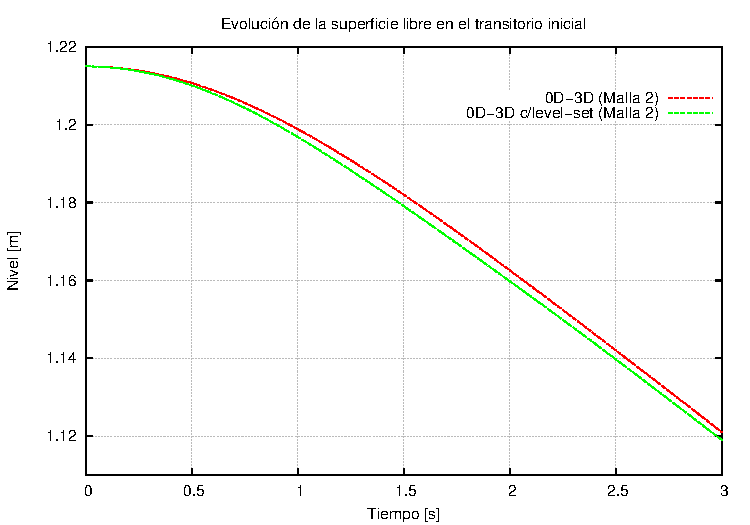
\includegraphics[scale = 1]{hvstlsZoom.pdf}
\caption{Evolución del nivel de líquido en el mockup del tanque del reflector ante accionamiento del SSP durante el transitorio inicial.
  Se comparan la solución obtenida despreciando el gas en la cañería y la obtenida con transporte de superficie libre mediante la técnica de \textit{level-set}.}  
	\label{hvstls}
\end{figure}

En la Figura \ref{evol-ls} se observa la evolución de la superficie libre durante los primeros instantes de tiempo.

\begin{figure}[ht]
\begin{minipage}[t]{.48\textwidth}
\centering
\subfloat[t = 0 s]{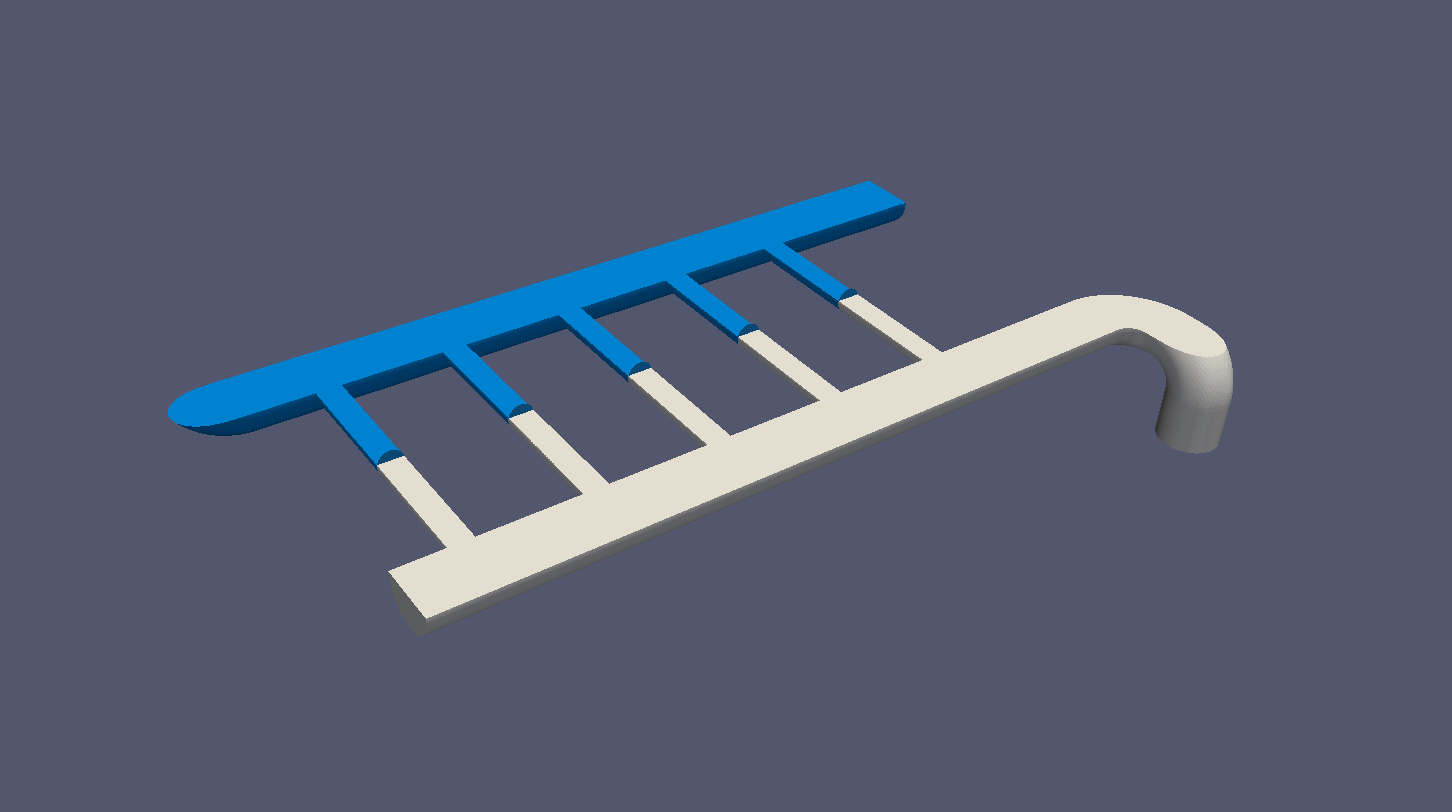
\includegraphics[scale=0.15]{0ms.png}}\\
\subfloat[t = 0.6 s]{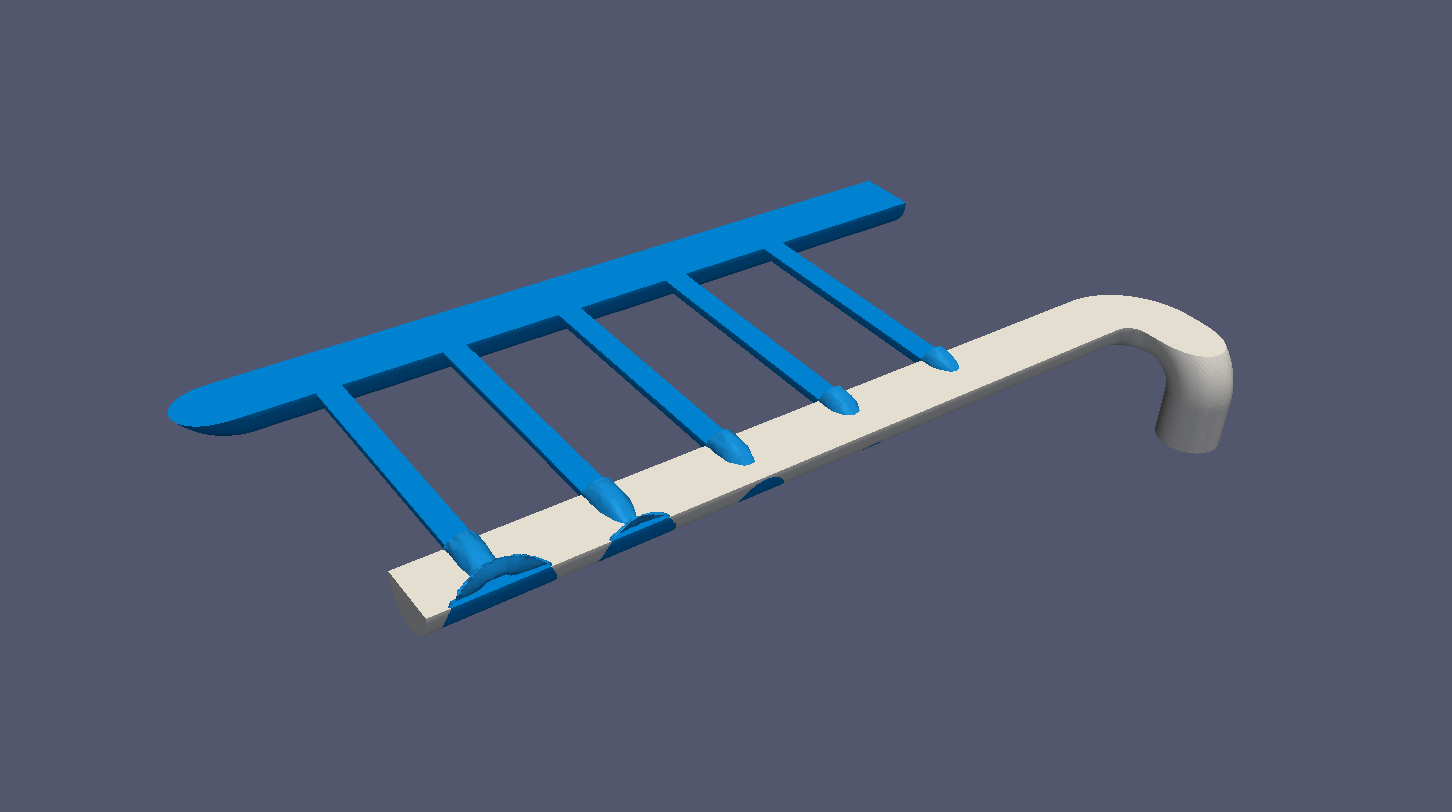
\includegraphics[scale=0.15]{600ms.png}}\\
\subfloat[t = 1.2 s]{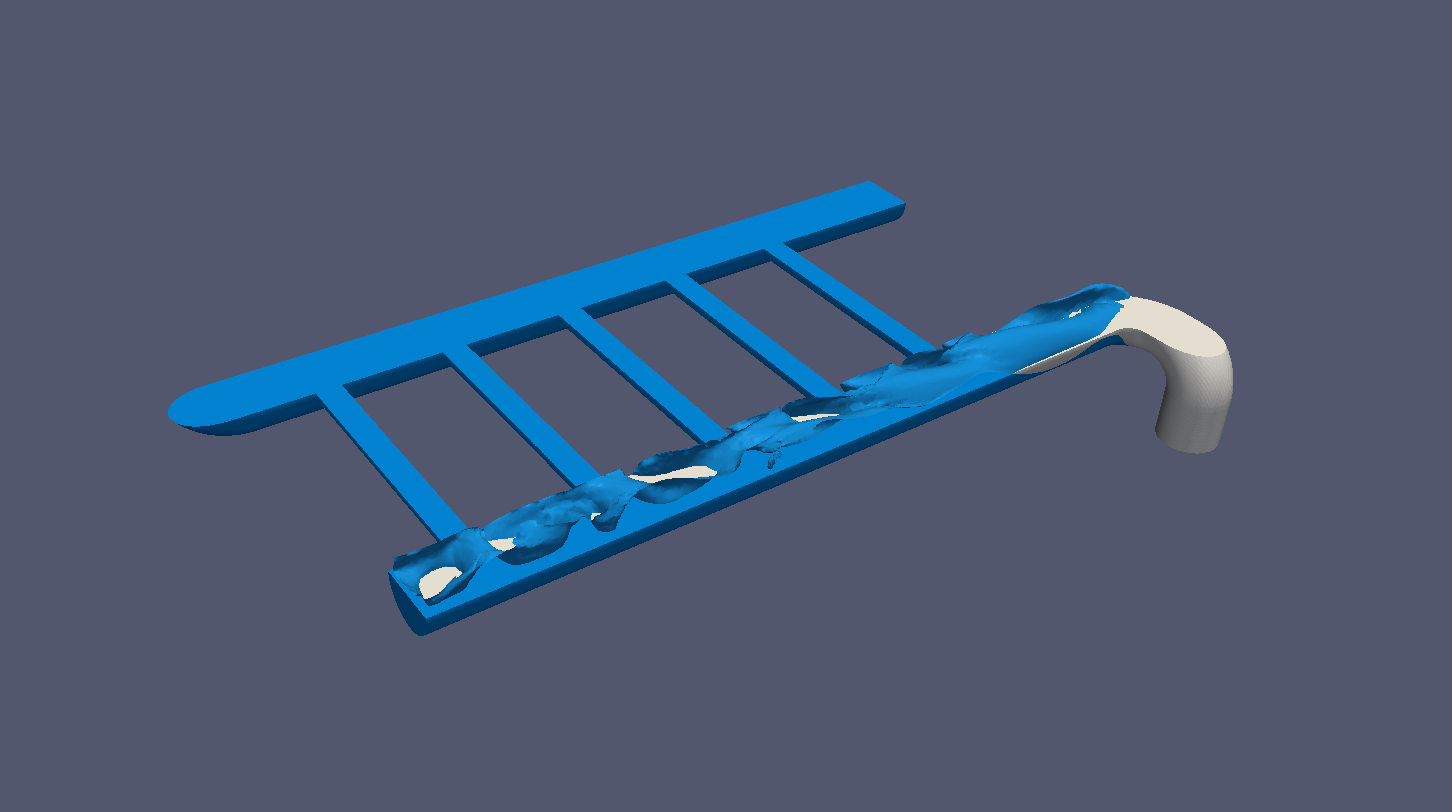
\includegraphics[scale=0.15]{1200ms.png}}
\end{minipage}\hfill
\begin{minipage}[t]{.48\textwidth}
\centering
\subfloat[t = 0.3 s]{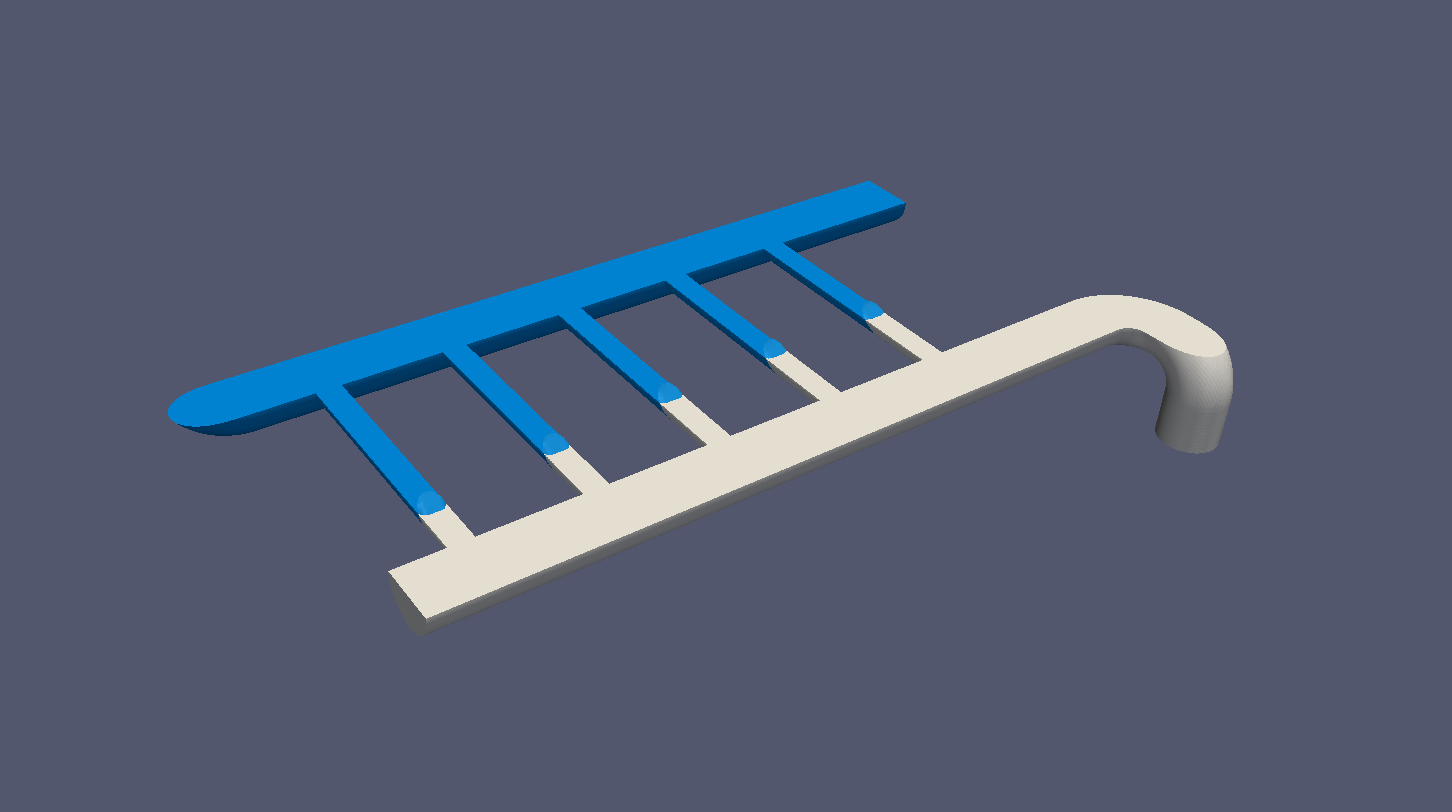
\includegraphics[scale=0.15]{300ms.png}}\\
\subfloat[t = 0.9 s]{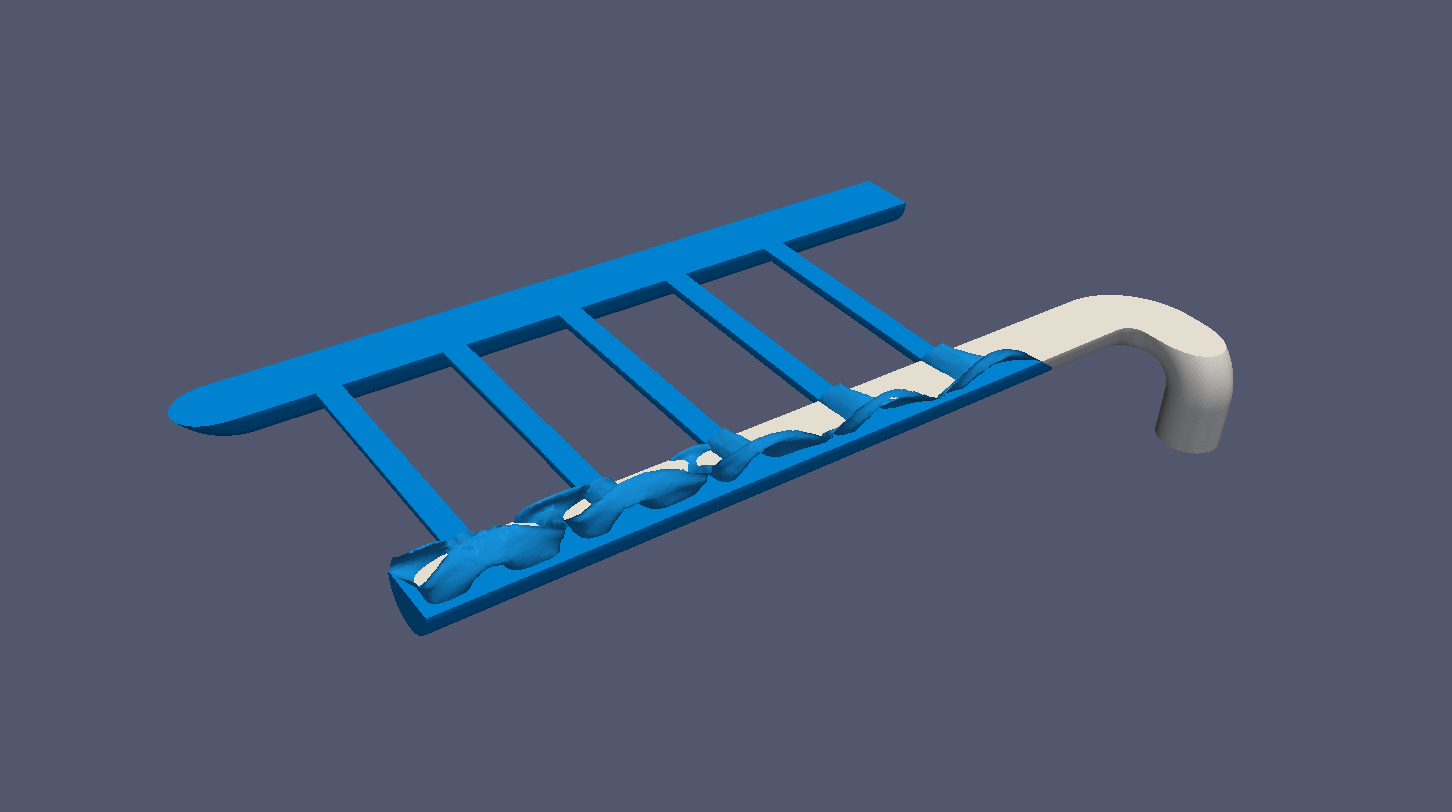
\includegraphics[scale=0.15]{900ms.png}}\\
\subfloat[t = 2.0 s]{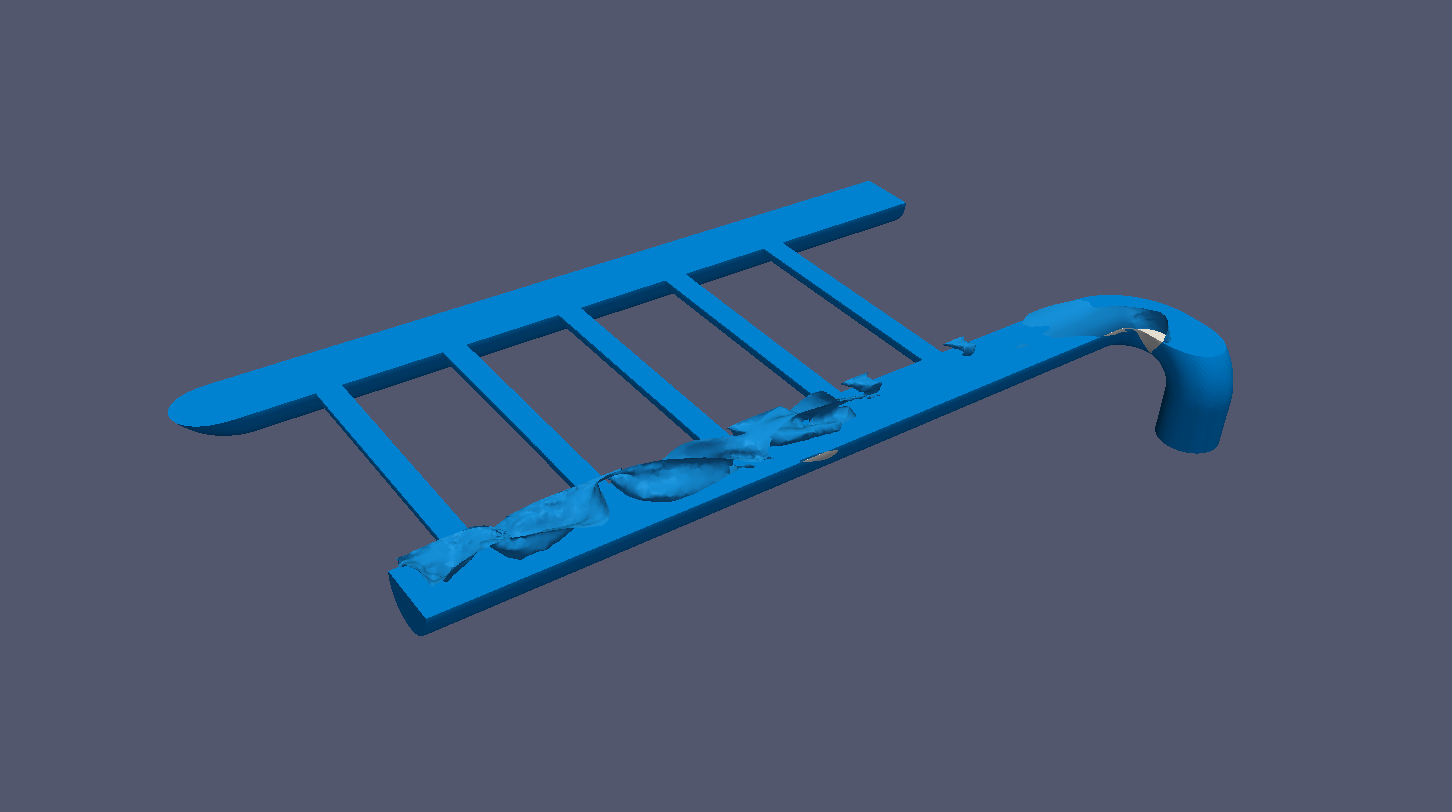
\includegraphics[scale=0.15]{2000ms.png}}
\end{minipage}
\caption{Transitorio inicial de la descarga del tanque a través del arreglo de válvulas, con falla simple en la última válvula
  (no se modela).
	El corte horizontal en la geometría permite observar el detalle de la evolución de la superficie libre.
  El líquido (azul) se encuentra inicialemente en condición estática rellenando las cañerías hasta la posición de las válvulas.
  Al otro lado el gas (blanco) rellena el resto de la red hidráulica.}  
\label{evol-ls}
\end{figure}

\subsection*{Conclusiones del análisis}
La herramienta de análisis de acoplamiento fuerte de subsistemas permite incorporar el estudio de la inercia fluídica en la red hidráulica de descarga.
Este estudio concluye que los modelos que incluyen el fenómeno inercial del fluido en la red hidráulica predicen un retraso de la descarga en un máximo de un segundo 
respecto a los modelos que no lo incluyen.
Como la inclusión del efecto inercial modela una dinámica similar a la reportada experimentalmente durante el transitorio inicial y,
además, es conservativa en función del objetivo de estudio establecido, debería ser considerada en futuros análisis de seguridad.

\subsection*{Análisis de métodos de resolución del sistema de ecuaciones de residuos}



\begin{figure}[ht]
\centering
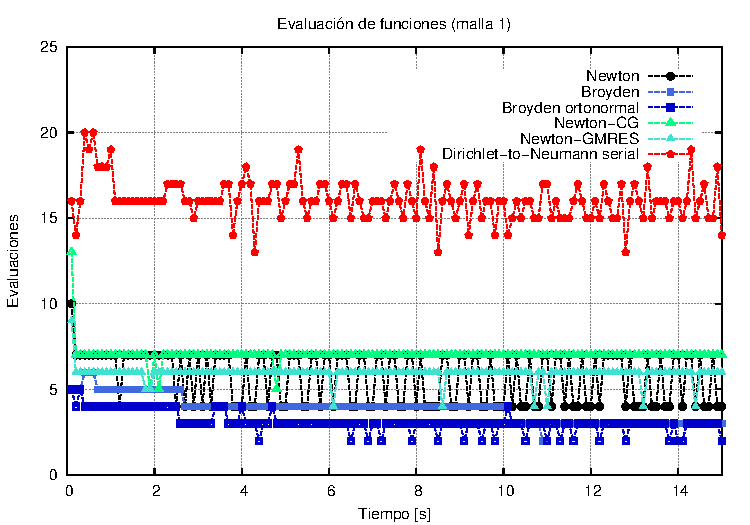
\includegraphics[scale = 1]{nonlinear_fevals.pdf}
\caption{.}  
	\label{nonlinear_fevals}
\end{figure}

\begin{figure}[ht]
\centering
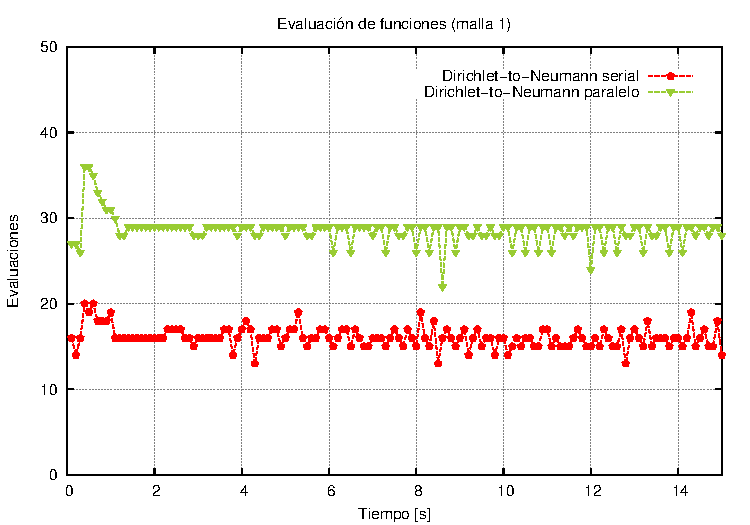
\includegraphics[scale = 1]{nonlinear_fevals_d2n.pdf}
\caption{.}  
	\label{nonlinear_fevals_d2n}
\end{figure}

\begin{figure}[ht]
\centering
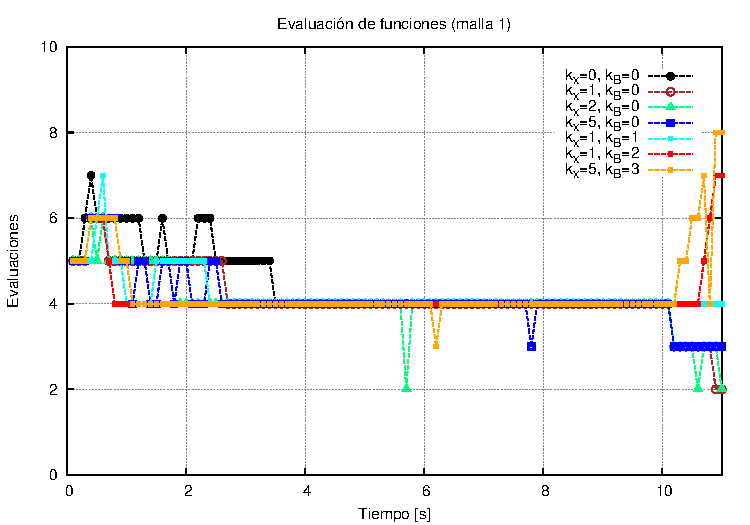
\includegraphics[scale = 1]{nonlinear_fevals_ex.pdf}
\caption{.}  
	\label{nonlinear_fevals_ex}
\end{figure}






\section{Resolución de redes hidráulicas de múltiples componentes}
\label{3:redes}

Laminar flow

\begin{figure}[ht]
\centering
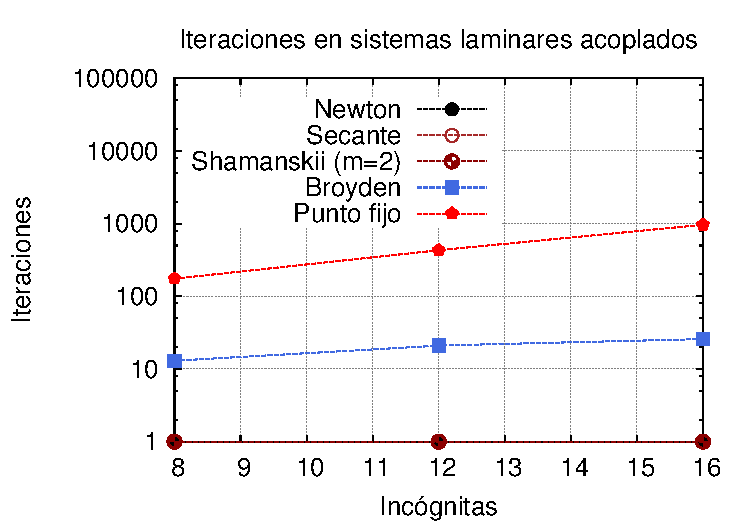
\includegraphics[scale = 1]{net_linear_its.pdf}
\caption{.}  
	\label{net_linear_its}
\end{figure}

\begin{figure}[ht]
\centering
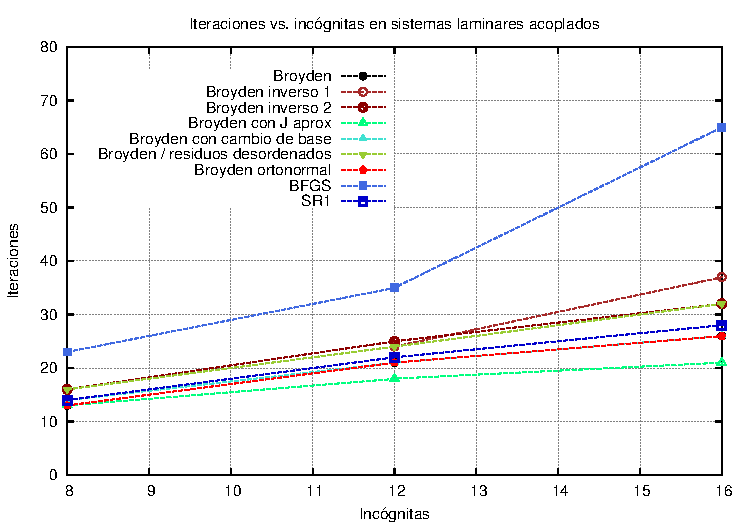
\includegraphics[scale = 1]{net_linear_fevals_broy.pdf}
\caption{.}  
	\label{net_linear_fevals_broy}
\end{figure}

\begin{figure}[ht]
\centering
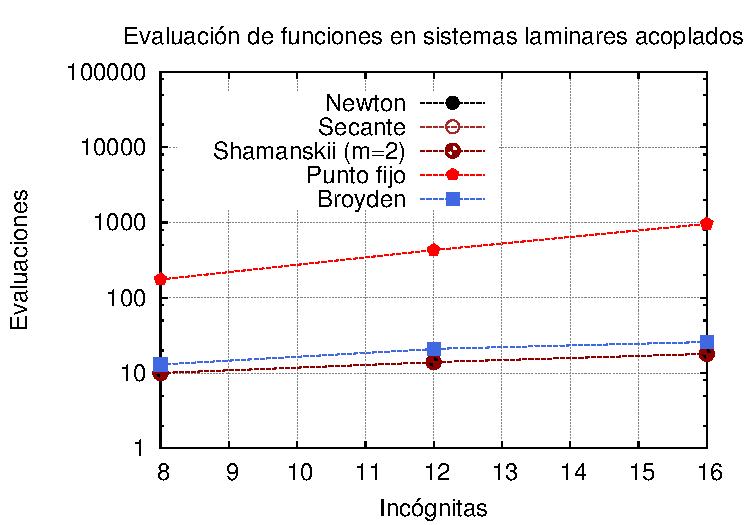
\includegraphics[scale = 1]{net_linear_fevals.pdf}
\caption{.}  
	\label{net_linear_fevals}
\end{figure}


Turbulent flow

\begin{figure}[ht]
\centering
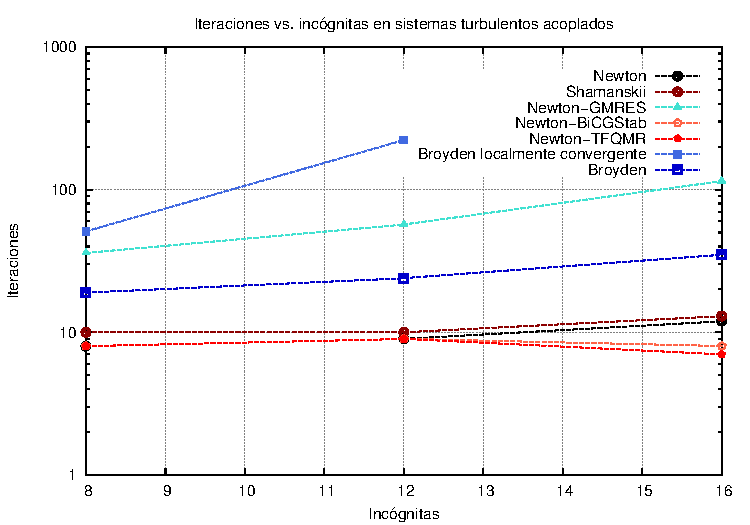
\includegraphics[scale = 1]{net_nonLinear_its.pdf}
\caption{.}  
	\label{net_nonLinear_its}
\end{figure}

\begin{figure}[ht]
\centering
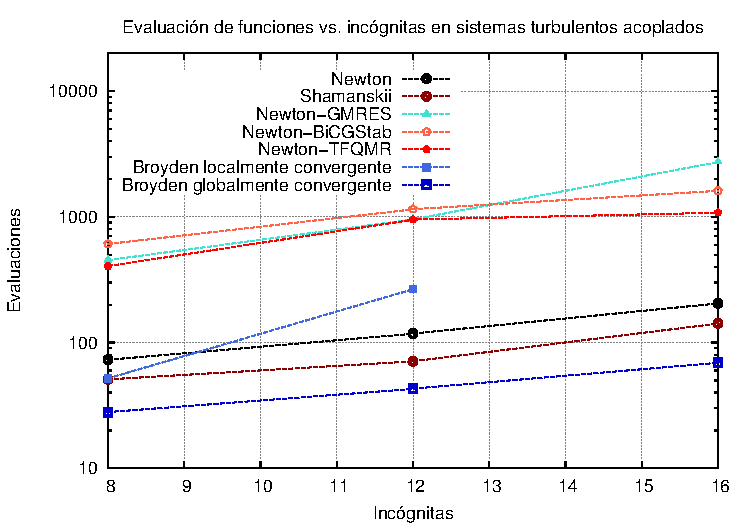
\includegraphics[scale = 1]{net_nonLinear_fevals.pdf}
\caption{.}  
	\label{net_nonLinear_fevals}
\end{figure}

\section{Extensión al problema neutrónico-termohidráulico}
\label{3:nt}

\subsection*{Estrategia de acoplamiento extendida}
\label{3:strategy-extended}
